% ============================================================
% Chapter 4 -- The rotating ring
%
% Original work of this thesis, reported here for the first time; there is
% no external source to cite for the derivations, the diagnostics, or the
% measurements.
% Numerical values are those of research/experiment1-rotating-ring/data.
% ============================================================

\chapter{The Rotating Ring: A Two-Dimensional Dynamic Object}
\label{ch:ring}

This is where the work started.

The object is a planar trajectory near a circle: a point that rotates by a
fixed angle each step, held near the unit radius by a confining drift, and
observed through the Ornstein--Uhlenbeck channel of
Section~\ref{sec:sm-diffusion}. It is a dynamic object in the sense of
Chapter~\ref{ch:model}, but a nonlinear one, and it was chosen before the
scalar chain precisely because rotation is a simple dynamic whose
signature is not visible in a single frame.

\section{Model and notation}\label{sec:ring-model}

\subsection{The clean process}

The clean state is a radius and a phase, evolving in the internal time $u$ as
two independent diffusions,
\begin{align}
  \dd R_u &= -\kappa (R_u - 1)\,\dd u + \sqrt{2 D_r}\, \dd B_u^{(r)} ,
  \label{eq:ring-radial-sde} \\
  \dd \Theta_u &= \omega\, \dd u + \sqrt{2 D_\theta}\, \dd B_u^{(\theta)} ,
  \label{eq:ring-angular-sde}
\end{align}
observed through the polar embedding
\begin{equation}
  a_u = R_u \big(\cos\Theta_u,\ \sin\Theta_u\big) \in \R^2 .
  \label{eq:ring-embedding}
\end{equation}
We use the simplest constant-angular-drift reading of the model; richer
readings --- state-dependent drift, coupled radius and phase --- change none of
the structural conclusions below and are not pursued.

A point of $\R^2$ is described by its distance from the origin and the angle it
makes with the first axis, and at each point the plane carries the orthonormal
moving frame
\begin{equation}
  e_r = (\cos\theta,\ \sin\theta), \qquad
  e_\theta = (-\sin\theta,\ \cos\theta) ,
  \label{eq:ring-moving-frame}
\end{equation}
in which $e_\theta$ is $e_r$ turned by a quarter revolution. Moving along $e_r$
changes the radius at fixed angle, moving along $e_\theta$ changes the angle at
fixed radius, and the area element is $\dd x\,\dd y = r\,\dd r\,\dd\theta$. The
decomposition matters because the two directions are treated very differently
by \eqref{eq:ring-radial-sde} and \eqref{eq:ring-angular-sde}: the radius is
pulled back towards one, the phase drifts and diffuses freely.

\subsection{The radial drift is a confining force}

Equation~\eqref{eq:ring-radial-sde} is an overdamped Langevin equation,
$\dd x_u = -\nabla V(x_u)\,\dd u + \sqrt{2D}\,\dd B_u$, for the quadratic
potential
\begin{equation}
  V(r) = \tfrac{\kappa}{2}\,(r-1)^2 .
  \label{eq:ring-potential}
\end{equation}
A potential stores energy, and the force it generates is minus its slope,
\begin{equation}
  F(r) = -V'(r) = -\kappa\,(r-1) .
  \label{eq:ring-force}
\end{equation}
The sign carries the content: along the \emph{deterministic} drift flow
$\dot r = -V'(r)$ the energy descends,
$\tfrac{\dd}{\dd u} V(r_u) = V'(r)\,\dot r = -V'(r)^2 \le 0$. Under the full
stochastic dynamics \eqref{eq:ring-radial-sde} It\^o's formula adds a
fluctuation source,
\begin{equation}
  \dd V(R_u)
  = \big[{-V'(R_u)^2} + D_r V''(R_u)\big]\,\dd u
  + \sqrt{2D_r}\,V'(R_u)\,\dd B_u^{(r)},
  \label{eq:ring-ito-energy}
\end{equation}
so $V$ is decreasing only on average and only away from the minimum; the
descent statement is a property of the drift, not of sample paths. Reading the
two cases of \eqref{eq:ring-force}, if $r > 1$ then $F < 0$ and the force points
inward, and if $r < 1$ then $F > 0$ and it points outward. The radius is driven
towards one from either side at a rate proportional to the displacement, with
$\kappa$ setting the stiffness. Overdamped Langevin dynamics equilibrates to
$p_\infty \propto e^{-V/D}$, so the stationary radial law is
$\Nd(1, D_r/\kappa)$.

One modelling caveat belongs here rather than in a footnote. A Gaussian law on
$\R$ puts mass on $R_u < 0$, so \eqref{eq:ring-radial-sde} defines a
\emph{signed} radial coordinate, not a geometric radius: through the embedding
\eqref{eq:ring-embedding} a negative $R_u$ is the point at radius $|R_u|$ and
phase $\Theta_u + \pi$. A strictly positive radius would require a reflected
or Bessel-type process with a repulsive $1/R$ It\^o term. We keep the linear
SDE because it is exactly solvable and because, in the confining regime
$D_r \ll \kappa$ used throughout, the stationary probability of a negative
coordinate, $\Phi(-\sqrt{\kappa/D_r})$, is negligible --- below $10^{-6}$
already at $\kappa/D_r = 23$ --- so origin crossings play no role in anything
measured here.

\subsection{One trajectory is one data point}

The trajectory is sampled at internal times $u_k = k h$ for
$k = 0, \dots, L-1$, and the complete datum is the stacked vector
\begin{equation}
  a = (a_0, a_1, \dots, a_{L-1}) \in \R^{2L} .
  \label{eq:ring-datum}
\end{equation}
The $L$ frames are correlated coordinates of one data point, not $L$ samples.
Relative to Chapter~\ref{ch:gaussian} the only change of setting is that each
frame is now two-dimensional, so the score has $L$ blocks of size two rather
than $L$ scalar components; the forward channel is unchanged,
\begin{equation}
  x = e^{-t} a + \sqrt{\Deltat}\, \xi , \qquad \xi \sim \Nd(0, I_{2L}) ,
  \label{eq:ring-channel}
\end{equation}
which is the channel of Section~\ref{sec:ou} acting on all $2L$ coordinates at
once. Figures~\ref{fig:ring-model-dynamics} and~\ref{fig:ring-model-channel} show
the model and the two clocks: internal time orders the frames along the path,
diffusion time corrupts them simultaneously.

\begin{figure}[t]
  \centering
  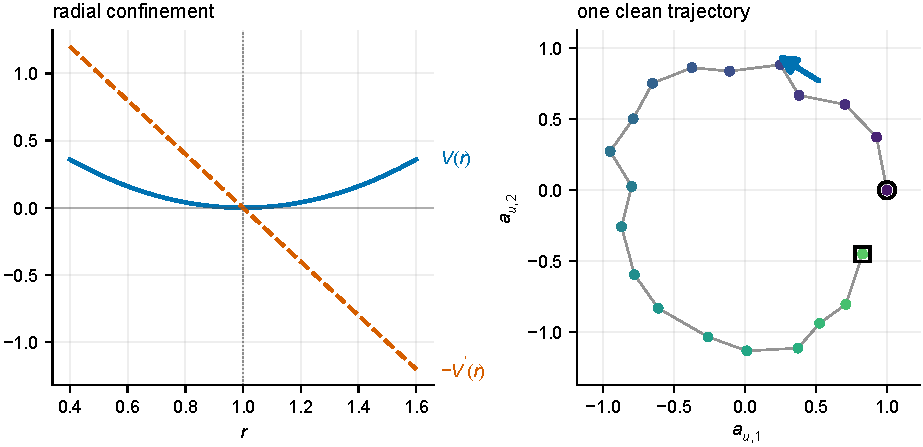
\includegraphics[width=\linewidth]{figures/fig_ring_model_dynamics.pdf}
  \caption[Radial confinement and angular motion]{%
    \textbf{Radial confinement and angular motion.}
    \textbf{(a)} The quadratic potential
    $V(r)=\frac{\kappa}{2}(r-1)^2$ has its minimum at $r=1$; the force
    $-V'(r)=-\kappa(r-1)$ points towards that stable radius from both sides.
    \textbf{(b)} One trajectory generated by the polar model.  Colour advances
    with the internal frame index; the open circle and square mark the first
    and final frames, respectively, and the curved arrow indicates the sense
    of the angular drift.}
  \label{fig:ring-model-dynamics}
\end{figure}

\begin{figure}[t]
  \centering
  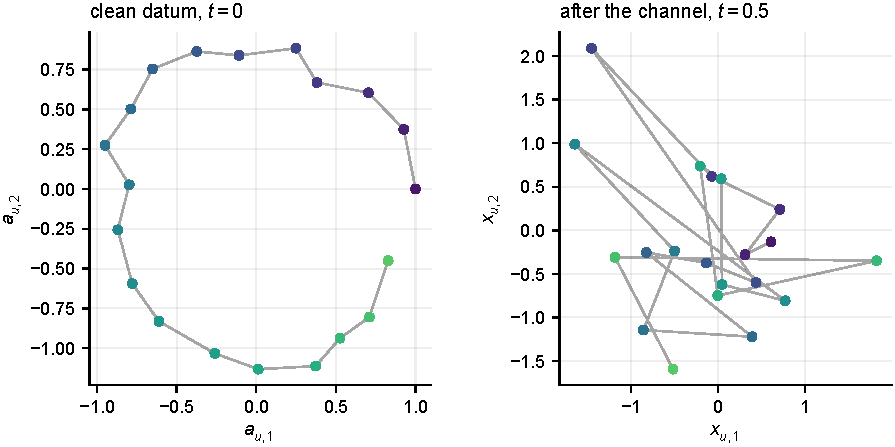
\includegraphics[width=\linewidth]{figures/fig_ring_model_channel.pdf}
  \caption[One rotating trajectory before and after the channel]{%
    \textbf{One trajectory before and after the Ornstein--Uhlenbeck channel.}
    \textbf{(a)} A clean datum consisting of $L=20$ ordered planar frames.
    \textbf{(b)} The same datum after independent coordinatewise corruption at
    diffusion time $t=0.5$.  Matching colours identify corresponding frame
    indices in the two panels.  The channel obscures the circular path, but the
    complete $2L$-dimensional trajectory remains the object whose joint score
    is sought.}
  \label{fig:ring-model-channel}
\end{figure}


\section{The gauge, and the exact score}\label{sec:ring-surrogate}

\subsection{The surrogate, and what it keeps}

The surrogate retains a ring, a coherent rotation, and dependence along the
trajectory, and drops the rest:
\begin{align}
  z_0 &\sim p_\lambda(z) \propto
        \exp\!\Big[-\frac{(\norm{z}-1)^2}{2\lambda}\Big] ,
  \label{eq:ring-sur-prior} \\
  z_{k+1} &= R_\psi z_k + \sigma \eta_{k+1} ,
        \qquad \eta_{k+1} \stackrel{\text{iid}}{\sim} \Nd(0, I_2) ,
  \label{eq:ring-sur-dynamics}
\end{align}
with $R_\psi$ the planar rotation through the one-frame angle
$\psi = \omega h$.

\begin{remark}[The surrogate is not a discretisation of the polar model]
\label{rem:ring-surrogate-scope}
In \eqref{eq:ring-sur-dynamics} the ring acts only on $z_0$. Later frames form
a rotating Cartesian random walk and their radial variance grows without bound,
whereas in \eqref{eq:ring-radial-sde} a confining force acts at every internal
time. The surrogate is a solvable companion whose role is to exhibit the
mechanism in closed form, not to approximate the model of
Section~\ref{sec:ring-model}.
\end{remark}

\subsection{The known rotation is an orthogonal change of frame}

The rotation is the object to be removed, so we write it out:
\begin{equation}
  R_\psi =
  \begin{pmatrix} \cos\psi & -\sin\psi \\ \sin\psi & \cos\psi \end{pmatrix} .
  \label{eq:ring-rotation}
\end{equation}
Its columns are the standard basis vectors, each turned through $\psi$. They
are unit vectors, since $\cos^2\psi + \sin^2\psi = 1$, and orthogonal, since
$\cos\psi(-\sin\psi) + \sin\psi\cos\psi = 0$. In matrix form,
\begin{equation}
  R_\psi^{\T} R_\psi = I_2, \qquad \det R_\psi = 1, \qquad
  R_\psi^{\T} = R_{-\psi}, \qquad R_\psi R_\varphi = R_{\psi+\varphi} ,
  \label{eq:ring-rot-props}
\end{equation}
and orthogonality gives
$\norm{R_\psi z}^2 = z^{\T} R_\psi^{\T} R_\psi z = \norm{z}^2$: lengths and
inner products are preserved.

\begin{lemma}[Rotations preserve the standard isotropic Gaussian]
\label{lem:ring-isotropy}
If $\eta \sim \Nd(0, I_2)$ and $R$ is orthogonal, then $R\eta \sim \Nd(0,I_2)$.
\end{lemma}

\begin{proof}
A linear map of a Gaussian is Gaussian, so $R\eta$ is fixed by its first two
moments: $\E[R\eta] = R\,\E[\eta] = 0$ and
$\mathrm{Cov}(R\eta) = R\, I_2\, R^{\T} = R R^{\T} = I_2$. Equivalently, in
terms of densities, $(2\pi)^{-1}e^{-\norm{z}^2/2}$ depends on $z$ only through
$\norm{z}$, and the change of variables $z \mapsto Rz$ changes neither
$\norm{R^{-1}z} = \norm{z}$ nor $|\det R^{-1}| = 1$: the level sets are circles
centred at the origin and a rotation maps each circle to itself.
\end{proof}

The isotropy is essential. A rotation would not preserve $\Nd(0,\Sigma)$ for
general $\Sigma$, and the reduction below is exact only because both the
innovation in \eqref{eq:ring-sur-dynamics} and the channel
\eqref{eq:ring-channel} are isotropic.

\begin{lemma}[Gauge reduction]\label{lem:ring-gauge}
Define the de-rotated frame $y_k = R_{-k\psi} z_k$ and stack the per-frame
rotations into
$U_\psi = \mathrm{diag}(I_2, R_{-\psi}, \dots, R_{-(L-1)\psi})$. Then
\begin{equation}
  y_{k+1} = y_k + \sigma \widetilde\eta_{k+1} ,
  \qquad \widetilde\eta_{k+1} \stackrel{\text{iid}}{\sim} \Nd(0, I_2) ,
  \label{eq:ring-gauged-rw}
\end{equation}
$U_\psi$ is orthogonal, and the noised density and score satisfy
\begin{equation}
  P_t(z \,|\, \psi) = P^{(0)}_t(U_\psi z) ,
  \qquad
  \score_\psi(z,t) = U_\psi^{\T}\, \score^{(0)}(U_\psi z, t) ,
  \label{eq:ring-gauge-score}
\end{equation}
where the superscript zero denotes the quantities of the non-rotating model.
\end{lemma}

\begin{proof}
Substituting \eqref{eq:ring-sur-dynamics} and using the composition rule of
\eqref{eq:ring-rot-props},
\begin{equation*}
  y_{k+1}
  = R_{-(k+1)\psi}\big(R_\psi z_k + \sigma\eta_{k+1}\big)
  = \underbrace{R_{-(k+1)\psi}R_\psi}_{= R_{-k\psi}} z_k
    + \sigma R_{-(k+1)\psi}\eta_{k+1}
  = y_k + \sigma\widetilde\eta_{k+1} ,
\end{equation*}
and by Lemma~\ref{lem:ring-isotropy} each
$\widetilde\eta_{k+1} \sim \Nd(0,I_2)$; they stay independent because each is a
fixed linear map of a different independent $\eta$. Next, $U_\psi$ is block
diagonal with orthogonal blocks, so
$U_\psi^{\T} U_\psi = \mathrm{diag}(I_2, \dots, I_2) = I_{2L}$ and
$\det U_\psi = \prod_k \det R_{-k\psi} = 1$. Applying $U_\psi$ to
\eqref{eq:ring-channel} gives
$U_\psi x = e^{-t} U_\psi a + \sqrt{\Deltat}\, U_\psi \xi$ with
$U_\psi \xi \sim \Nd(0, I_{2L})$, so $U_\psi x$ has exactly the law of the
noised non-rotating trajectory: the de-rotation commutes with the channel. For
the densities, $z = U_\psi^{\T} y$ and
$P_t(z\,|\,\psi) = P^{(0)}_t(U_\psi z)\,|\det U_\psi|$, the Jacobian factor
being one. Differentiating that identity componentwise, with
$\partial y_b/\partial z_c = (U_\psi)_{bc}$,
\begin{equation*}
  \frac{\partial}{\partial z_c} \log P^{(0)}_t(U_\psi z)
  = \sum_b (U_\psi)_{bc}\,
    \big(\nabla \log P^{(0)}_t\big)_b (U_\psi z)
  = \big[ U_\psi^{\T} \score^{(0)}(U_\psi z, t) \big]_c .
\end{equation*}
The transpose is not cosmetic: a score is a gradient, so it transforms with
$U_\psi^{\T}$ while a point transforms with $U_\psi$.
\end{proof}

Equation~\eqref{eq:ring-gauge-score} says that a known rotation adds
no statistical difficulty: de-rotate the data, solve the non-rotating problem,
rotate the score back. Since $U_\psi^{\T} = U_\psi^{-1}$, the operation is
exactly invertible and destroys no information. It would not hold for an
\emph{unknown} $\psi$, which is a genuine latent variable. Figure~\ref{fig:ring-gauge} shows the two
frames.

\begin{figure}[t]\centering

\includegraphics[width=\linewidth]{fig_ring_gauge.pdf}
\caption[The rotation as a gauge, before and after]{The rotation and the gauge. (a) $R_\psi$ turns every vector through
the same angle without changing its length, which is the statement
$R_\psi^{\T}R_\psi = I_2$. (b) Three surrogate trajectories in the laboratory
frame ($L = 14$, $\sigma = 0.16$, $\psi = 2\pi/14$; the marked point is
$k = 0$), coherently circulating. (c) The same trajectories after $U_\psi$: a
random walk anchored on the ring.}
\label{fig:ring-gauge}
\end{figure}

\subsection{Why the surrogate is worth solving}
\label{sec:ring-surrogate-meaning}

The surrogate's payoff is three closed-form objects:
\begin{align}
  S_k^{(0)}(\widetilde x,t)
    &= -\bigl(C_t^{-1}\widetilde x\bigr)_k
       + e^{-t}q_k\,\mathbb E[A\mid\widetilde x],
    \label{eq:ring-recap-score}\\
  J_{kj}^{(0)}(\widetilde x,t)
    &= -\bigl(C_t^{-1}\bigr)_{kj} I_2
       + e^{-2t}q_kq_j\operatorname{Cov}(A\mid\widetilde x),
    \label{eq:ring-recap-response}\\
  S_\psi(x,t) &= U_\psi^{\mathsf T}S^{(0)}(U_\psi x,t),
    \label{eq:ring-recap-gauge}
\end{align}
the exact score and response of the de-rotated surrogate, and the gauge map
that carries them back to the laboratory frame. The first two are new; the
third is Lemma~\ref{lem:ring-gauge} restated for the anchor-marginalised
law, not a further derivation. The derivation of
\eqref{eq:ring-recap-score}--\eqref{eq:ring-recap-response} is
Toolbox~\ref{tb:ring-exact-score}.


\begin{toolbox}[tb:ring-exact-score]{From the anchor posterior to the exact
score and response}

In the de-rotated frame the surrogate is the anchored random walk
\eqref{eq:ring-gauged-rw}: $y_0 = A$ and
$y_k = A + \sigma\sum_{r=1}^{k}\widetilde\eta_r$. Conditionally on the
anchor the walk increments are the only randomness, so
$\operatorname{Cov}(y_i, y_j \mid A) = \sigma^2 \min(i,j)\, I_2$ under the
zero-based indexing used here --- the first frame is pinned to the anchor
exactly, $\min(0, j) = 0$. Passing through the channel
\eqref{eq:ring-channel} scales the conditional covariance by $e^{-2t}$ and
adds white noise, which defines the matrix used throughout this toolbox:
\begin{equation}
  C_t := e^{-2t}\sigma^2 M + \Deltat I_L,
  \qquad
  M_{ij} = \min(i,j),
  \qquad i,j = 0,\dots,L-1,
  \label{eq:ring-Ct-def}
\end{equation}
positive definite for every $t > 0$ because of the $\Deltat I_L$ term even
though $M$ is singular. For $t>0$, conditionally on the anchor $A=\alpha$, the
de-rotated noisy trajectory is therefore Gaussian,
\begin{equation}
  \widetilde x \mid A=\alpha
  \sim
  \Nd\!\left(
    e^{-t}\mathbf 1\otimes\alpha,\,
    C_t\otimes I_2
  \right).
  \label{eq:ring-conditional-noised-law}
\end{equation}
Write
\begin{equation}
  q = C_t^{-1}\mathbf 1,
  \qquad
  h(\widetilde x)
  = e^{-t}(q^{\mathsf T}\otimes I_2)\widetilde x
  = e^{-t}\sum_{j=0}^{L-1} q_j\,\widetilde x_j .
  \label{eq:ring-anchor-statistic}
\end{equation}
Here and below the action of $C_t^{-1}$ on a block vector is understood as
\[
  \big[(C_t^{-1}\otimes I_2)\widetilde x\big]_k
  =
  \sum_{j=0}^{L-1}(C_t^{-1})_{kj}\widetilde x_j .
\]

\medskip
\noindent\textbf{Score.}
For a latent-variable model
\[
  p_t(\widetilde x)
  =
  \int p(\widetilde x\mid\alpha)\,p(\alpha)\,\dd\alpha,
\]
differentiation under the integral gives Fisher's identity,
\begin{equation}
  \nabla_{\widetilde x_k}\log p_t(\widetilde x)
  =
  \E\!\left[
    \nabla_{\widetilde x_k}
    \log p(\widetilde x\mid A)
    \,\middle|\,\widetilde x
  \right].
  \label{eq:ring-fisher-identity}
\end{equation}
For the Gaussian law \eqref{eq:ring-conditional-noised-law},
\begin{align}
  \nabla_{\widetilde x_k}
  \log p(\widetilde x\mid\alpha)
  &=
  -\big[(C_t^{-1}\otimes I_2)\widetilde x\big]_k
  +e^{-t}(C_t^{-1}\mathbf 1)_k\,\alpha
  \nonumber\\
  &=
  -\sum_{j=0}^{L-1}(C_t^{-1})_{kj}\widetilde x_j
  +e^{-t}q_k\,\alpha .
  \label{eq:ring-conditional-score}
\end{align}
Averaging over the anchor posterior therefore gives
\begin{equation}
  \boxed{
  S_k^{(0)}(\widetilde x,t)
  =
  -\sum_{j=0}^{L-1}(C_t^{-1})_{kj}\widetilde x_j
  +e^{-t}q_k\,\E[A\mid\widetilde x]
  }.
\end{equation}

\medskip
\noindent\textbf{Response.}
Expanding the Gaussian exponent in
\eqref{eq:ring-conditional-noised-law} shows that the dependence of the
anchor posterior on the full trajectory is only through the two-dimensional
statistic $h(\widetilde x)$:
\begin{equation}
  p(\alpha\mid\widetilde x)
  \propto
  \exp\!\left\{
    g_t(\alpha)+h(\widetilde x)^{\mathsf T}\alpha
  \right\},
  \label{eq:ring-anchor-posterior}
\end{equation}
where $g_t$ contains the prior and all terms independent of
$\widetilde x$ once $h$ is fixed.

Let
\[
  Z(h)=\int
  \exp\!\left\{g_t(\alpha)+h^{\mathsf T}\alpha\right\}
  \dd\alpha .
\]
Then the posterior mean is
\[
  m(h)
  :=
  \E[A\mid h]
  =
  \nabla_h\log Z(h),
\]
and its Jacobian is the posterior covariance,
\begin{equation}
  \nabla_h m(h)
  =
  \nabla_h^2\log Z(h)
  =
  \Cov(A\mid h).
  \label{eq:ring-mean-covariance-identity}
\end{equation}
Since
\[
  \frac{\partial h}{\partial\widetilde x_j}
  =
  e^{-t}q_j I_2,
\]
the chain rule gives
\begin{equation}
  \frac{\partial}{\partial\widetilde x_j}
  \E[A\mid\widetilde x]
  =
  e^{-t}q_j\,\Cov(A\mid\widetilde x).
  \label{eq:ring-anchor-response}
\end{equation}
Differentiating \eqref{eq:ring-recap-score} once more therefore yields
\begin{equation}
  \boxed{
  J_{kj}^{(0)}(\widetilde x,t)
  =
  -(C_t^{-1})_{kj}I_2
  +
  e^{-2t}q_kq_j\,
  \Cov(A\mid\widetilde x)
  }.
\end{equation}

Equivalently, for the complete $2L$-dimensional score and response,
\begin{align}
  S^{(0)}(\widetilde x,t)
  &=
  -(C_t^{-1}\otimes I_2)\widetilde x
  +e^{-t}(q\otimes I_2)\E[A\mid\widetilde x],
  \label{eq:ring-score-vector-form}\\
  J^{(0)}(\widetilde x,t)
  &=
  -(C_t^{-1}\otimes I_2)
  +e^{-2t}
   \bigl(qq^{\mathsf T}\otimes
   \Cov(A\mid\widetilde x)\bigr).
  \label{eq:ring-response-vector-form}
\end{align}
Thus marginalising a single two-dimensional anchor modifies the Gaussian
response through a term that is rank one in the frame indices and has rank at
most two in the full $2L$-dimensional space.
\end{toolbox}

Three things follow from having these in closed form rather than as an
intractable integral. It gives an exact score to check numerical inference
against. It identifies the sufficient statistic: every frame feeds into $h$,
but all the remaining nonlinearity concerns only the two-dimensional anchor
$A$, not the full $2L$-dimensional trajectory. And it separates two
mechanisms inside the response $J_{kj}^{(0)}$: the $C_t^{-1}$ term is the
ordinary Gaussian-walk covariance, while the rank-one term $q_kq_j$ is what
one shared latent variable, marginalised, does to every pair of frames at
once. This structured loss of locality is what
carries over to the model that cannot be solved in closed form.

\section{Does the score know the data are rotating?}
\label{sec:ring-return-original}

 With a uniform initial phase, one
frame's law is a rotationally symmetric annulus --- it does not itself look
like "a rotation." Rotation is a property of the transition law between
ordered frames, not of any single frame's distribution. So the question
is: given only the noised data, does the score --- built without
ever being told the generative process turns --- carry a usable signal that
it does, and if so, where does that signal live?

\subsection{One frame: no}
\label{sec:ring-marginal-blindness}

\begin{theorem}[Marginal blindness]
\label{thm:ring-marginal-blindness}
With the initial phase uniform on the circle, every one-frame marginal is
independent of the angular drift, at every diffusion time. This holds for
the polar model in $\omega$ and for the surrogate in $\psi$. Consequently,
every one-frame score carries zero Fisher information about the rotation.
\end{theorem}

\begin{proof}
For the polar model, $\Theta_u=\Theta_0+\omega u+\sqrt{2D_\theta}\,B_u^{(\theta)}$.
Adding any independent angle to a uniform circular variable returns a
uniform variable, so $\Theta_u$ is uniform for every $u$ and every $\omega$;
$R_u$ carries no $\omega$ and is independent of $\Theta_u$, so the law of
$a_u=R_u(\cos\Theta_u,\sin\Theta_u)$ does not depend on $\omega$ either. The
surrogate's initial law and Gaussian innovations are rotationally invariant
for the same reason, and the channel is isotropic and parameter-free, so
noising preserves the independence. Hence $\partial_\omega\log p_t(x_u)=0$
and $\partial_\psi\log p_t(x_u)=0$ for every frame and every $t$.
\end{proof}


Therefore, as expected, no amount of per-frame looking, however much data, recovers the one thing
rotation is: a direction of turning.

\subsection{The trajectory: yes, and here is how}
\label{sec:ring-how-score-contains-rotation}

The mechanism is visible in closed form for the clean surrogate.
The derivation is Toolbox~\ref{tb:ring-score-rotation}; for an interior
frame it gives
\begin{equation}
  S_k(z,0)
  =\frac{1}{\sigma^2}
  \left(
    R_\psi z_{k-1}
    +R_\psi^{\mathsf T}z_{k+1}
    -2z_k
  \right).
  \label{eq:ring-rotation-in-score}
\end{equation}

\begin{toolbox}[tb:ring-score-rotation]{The clean surrogate score at an
interior frame}
The joint law of the clean surrogate factorises along the chain,
\[
  p(z_0,\dots,z_{L-1})
  = p_\lambda(z_0)\prod_{i=0}^{L-2}
    \Nd\big(z_{i+1};\,R_\psi z_i,\,\sigma^2 I_2\big),
\]
so, up to additive terms not involving $z_k$,
\[
  \log p(z)
  =
  -\frac{1}{2\sigma^2}\big\lVert z_k - R_\psi z_{k-1}\big\rVert^2
  -\frac{1}{2\sigma^2}\big\lVert z_{k+1} - R_\psi z_k\big\rVert^2
  + \mathrm{const}.
\]
For an interior frame $1\le k\le L-2$, $z_k$ appears in exactly these two
terms --- once as the point being predicted from $z_{k-1}$, once as the
point doing the predicting of $z_{k+1}$ --- and nowhere else, since
$p_\lambda(z_0)$ does not involve $z_k$ when $k\neq0$.

\emph{The first term.} Differentiating directly,
\[
  \nabla_{z_k}\left[-\frac{1}{2\sigma^2}\lVert z_k-R_\psi z_{k-1}\rVert^2\right]
  = -\frac{1}{\sigma^2}\big(z_k - R_\psi z_{k-1}\big).
\]

\emph{The second term.} Writing $u = z_{k+1}-R_\psi z_k$, the Jacobian of
$u$ with respect to $z_k$ is $-R_\psi$, so
$\nabla_{z_k}\lVert u\rVert^2 = 2(-R_\psi)^{\mathsf T}u$, and
\[
  \nabla_{z_k}\left[-\frac{1}{2\sigma^2}\lVert z_{k+1}-R_\psi z_k\rVert^2\right]
  = \frac{1}{\sigma^2}R_\psi^{\mathsf T}\big(z_{k+1}-R_\psi z_k\big)
  = \frac{1}{\sigma^2}\Big(R_\psi^{\mathsf T}z_{k+1} - z_k\Big),
\]
using $R_\psi^{\mathsf T}R_\psi = I_2$ from \eqref{eq:ring-rot-props} to
collapse $R_\psi^{\mathsf T}R_\psi z_k$ to $z_k$.

\emph{Adding the two.} $S_k(z,0)=\nabla_{z_k}\log p(z)$ is the sum of both
contributions:
\[
  S_k(z,0)
  = \frac{1}{\sigma^2}\Big[-z_k + R_\psi z_{k-1}\Big]
  + \frac{1}{\sigma^2}\Big[R_\psi^{\mathsf T}z_{k+1} - z_k\Big]
  = \frac{1}{\sigma^2}\Big(R_\psi z_{k-1} + R_\psi^{\mathsf T}z_{k+1} - 2z_k\Big),
\]
which is \eqref{eq:ring-rotation-in-score}. \hfill$\square$
\end{toolbox}

Therefore, the score at frame $k$ does not compare $z_k$ to
its neighbours directly, it compares $z_k$ to the previous frame rotated
forward by one step and the next frame rotated back by one step.
The polar model cannot be reduced this cleanly, but the same mechanism
operates through the posterior. The $k$-th joint-score block is the
denoising identity
\begin{equation}
  S_{\omega,k}(x,t)
  =\frac{e^{-t}\mathbb E_\omega[a_k\mid x]-x_k}{\Delta_t},
  \label{eq:ring-polar-denoising-score}
\end{equation}
where
\begin{equation}
  p_\omega(a\mid x)
  \propto
  p(a_0)
  \prod_{u=0}^{L-2}K_\omega(a_{u+1}\mid a_u)
  \prod_{u=0}^{L-1}
  \mathcal N(x_u;e^{-t}a_u,\Delta_t I_2).
  \label{eq:ring-polar-posterior}
\end{equation}
$K_\omega$ favours angular increments consistent with the drift, so it pulls
the posterior mean of $a_k$ away from "wherever $x_k$ alone suggests" and
towards "wherever the neighbouring frames say a turning trajectory should
be."

Two scope notes complete the statement. The parameter enters only through the
one-step rotation, so from discrete frames it is identifiable at most modulo
$2\pi$ in the per-step angle ($\psi$ and $\psi + 2\pi$ generate identical
laws); within a fundamental interval $(-\pi, \pi]$ the joint law does
distinguish $\psi$ from $-\psi$, which is the sense in which the direction of
turning is knowable. And what this section establishes is that the joint law
\emph{carries information} about the drift --- the marginal Fisher information
is zero while the joint likelihood depends on $\omega$ --- not a recovery
theorem: no estimator of $\omega$, and no rate, is constructed here.

\section{Chapter conclusion}
\label{sec:ring-conclusion}

The rotating ring separates two kinds of information that a static object
never distinguishes. The one-frame score reports where probability mass
sits --- here, an annulus. The joint score also reports how frames relate
to one another --- here, an oriented turn through internal time, invisible
to any one frame and identifiable (modulo the angular aliasing above) from the
joint law of the trajectory.

The surrogate is what makes this exact: its
score is a Gaussian-walk term plus a rank-one correction generated by one
shared unknown, and the gauge shows precisely how the sense of rotation
enters through forward and backward comparisons between frames. Returning
to the polar model shows the same split holding at the level of information
itself: every one-frame marginal is exactly blind to $\omega$; the joint
law carries information identifying it through the transition kernel, until
the noise wins.

\begin{equation}
  \boxed{
  \begin{aligned}
    \text{one-frame score}
      &\;\longrightarrow\;\text{geometry},\\
    \text{joint trajectory score}
      &\;\longrightarrow\;\text{geometry and dynamics}.
  \end{aligned}}
  \label{eq:ring-chapter-message}
\end{equation}